\section{Introduction}\label{sec:intro}
Experiments on social networks and marketplaces violate the assumption that a unit's outcome depends only on its own treatment. A decision-maker usually needs the global average treatment effect (GATE), the difference between a world in which everyone is treated and one in which no one is, and a randomised experiment realises neither.
Two families of estimators recover it. Design-based estimators reweight the units that satisfy an exposure condition such as ``the unit and all its neighbours are treated'' \citep{aronow2017estimating}; they are unbiased when the condition is right, and their variance grows exponentially with degree, which cluster designs offset at a cost \citep{ugander2013graph}. Regression estimators fit the outcome on a unit's own treatment and a summary of its neighbours' treatments, and predict with everyone treated and everyone in control \citep{chin2019regression,han2023model}. They are cheap and widely used, and their error is understood only when the fitted model is correct.

This paper asks how accurate regression GATE estimators are, what determines their error, and where they hold or fail.
Our answer is that regression GATE estimation is \emph{extrapolation to the corner}. Under Bernoulli($p$) assignment a unit's treated-neighbour fraction $g$ concentrates around $p$, within $\sqrt{p(1-p)/d}$ for degree $d$, so the data never show $g=0$ or $g=1$, which is where the estimator evaluates its fit (Figure~\ref{fig:corner}). Its error is then the sum of a variance that grows as $\sqrt d$ and a bias, the gap between the chord that joins the two corners and the best-fitting line, that is set by the curvature of the true response and does not shrink with the sample size.
\begin{figure}[tb]
\centering
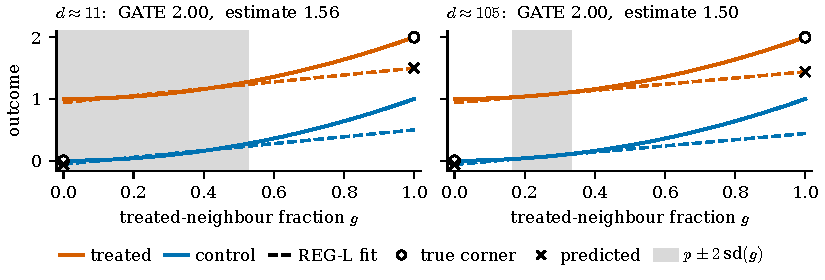
\includegraphics[width=\linewidth]{fig1_corner.pdf}
\caption{The corner is outside the data. One draw on an ER graph with $n=10^4$ ($p=0.25$, convex response, $\gate=2$) at two mean degrees. Curves: true outcomes of treated and control units against the treated-neighbour fraction $g$; dashed: the line \est{REG-L} fits; shaded: where the data lie, $p\pm2\,\mathrm{sd}(g)$; circle and cross: true and predicted outcome at $g=0$ and $g=1$.}
\label{fig:corner}
\end{figure}

We test this account on a simulation family with continuous curvature, range and effect size and a fixed truth $\gate=2$ (Section~\ref{sec:setup}), on synthetic graphs and two real Facebook graphs with synthetic outcomes. Our contributions are:
\begin{itemize}
\item \textbf{An error anatomy that predicts what we measure.} With the right model, the standard deviation equals $\sqrt{\sigma^2L/n}$ for the corner leverage $L$ (ratio 0.90--1.15 over 150 cells); with the wrong model, the bias equals the exact projection bias, computed from the graph and design alone (correlation 0.9996 over 320 cells), and does not fall with $n$.
\item \textbf{The competitor is the relaxed design-based estimator.} Regression beats exact Horvitz--Thompson (error $10^3$ at $d=20$) at every degree from two upward, and loses to relaxed-exposure Hájek or to ignoring interference only for step-like responses.
\item \textbf{One degree summary organises the error across graphs.} With the harmonic mean degree the variance follows $Z_0+Z_1$ without a fitted parameter ($R^2=0.97$) and a held-out graph family's bias is predicted with $R^2$ 0.90--0.97.
\item \textbf{A map of failures, with negative results.} Flexible regression does not remove the floor; an omitted two-hop term multiplies the error by five; three data-only scores of the bias do not beat the corner distance, and a fourth, which transports a low-degree fit, ranks the bias only where the response does not depend on degree; and a bias-aware interval covers only by being wide.
\end{itemize}
All results are for this simulation family, whose limits Section~\ref{sec:discussion} states. Code, data and a script for every figure and table are released with the paper.
